\chapter{Resultados}
Nessa capítulo, constará os gráficos e tabelas referentes aos resultados do experimento. Primeiro será apresentado os dados de cada um dos algoritmos e após uma visão geral.

\section{Resultados de cada algoritmo}
A seguir, poderá ser encontrado as tabelas e gráficos referentes as médias finais de cada algoritmo para sua respectiva entrada de elementos. O tempo foi medido em milissegundos. A primeira coluna consta a quantidade de elementos presente no arranjo, as outras 3 colunas constam, respectivamente, o tempo médio que o algoritmo levou para arranjos aleatórios, arranjos com elementos em ordem crescente e arranjos com elementos em ordem decrescente.

Em uma visão geral, podemos notar que os algoritmos realmente agem melhor nos arranjos ordenados crescentemente e que seus piores casos são quando o arranjo está ordenado em ordem decrescente.

\subsection{Insertion sort}
\begin{longtable}{|r|c|c|c|}
	\hline
	\csvreader[
		column count=5,
		no head,
		table head=\hline,
		late after line=\\\hline
	]{csvs/Insertion_Sort.csv}{
		1=\n-elementos, 2=\aleatorio, 3=\crescente, 4=\decrescente
	}{ \n-elementos & \aleatorio & \crescente & \decrescente }
	\caption{Média de tempo do Insertion Sort}
	\label{t-insertion}
\end{longtable}

\begin{figure}[H]
	\centering
	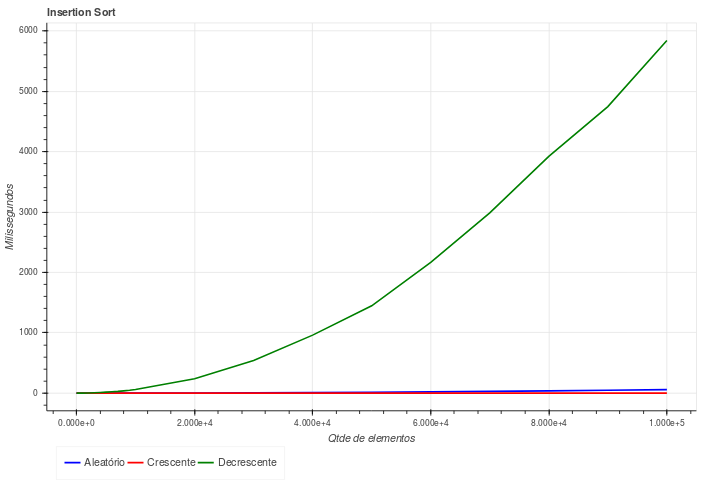
\includegraphics[scale=0.6]{img/algoritmos/insertion_sort.png}
	\caption{Insertion Sort, gráfico de resultados.}
	\label{graph-insertion}
\end{figure}

\subsection{Selection sort}
\begin{longtable}{|r|c|c|c|}
	\hline
	\csvreader[
		column count=5,
		no head,
		table head=\hline,
		late after line=\\\hline
	]{csvs/Selection_Sort.csv}{
		1=\n-elementos, 2=\aleatorio, 3=\crescente, 4=\decrescente
	}{ \n-elementos & \aleatorio & \crescente & \decrescente }
	\caption{Média de tempo do Selection Sort}
	\label{t-selection}
\end{longtable}

\begin{figure}[H]
	\centering
	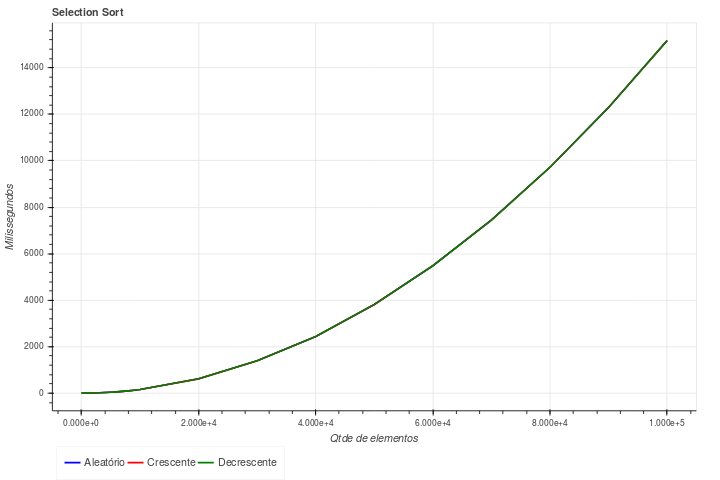
\includegraphics[scale=0.6]{img/algoritmos/selection_sort.png}
	\caption{Selection Sort, gráfico de resultados.}
	\label{graph-selection}
\end{figure}

\subsection{Bubble sort}
\begin{longtable}{|r|c|c|c|}
	\hline
	\csvreader[
		column count=5,
		no head,
		table head=\hline,
		late after line=\\\hline
	]{csvs/Bubble_Sort.csv}{
		1=\n-elementos, 2=\aleatorio, 3=\crescente, 4=\decrescente
	}{ \n-elementos & \aleatorio & \crescente & \decrescente }
	\caption{Média de tempo do Bubble Sort}
	\label{t-bubble}
\end{longtable}

\begin{figure}[H]
	\centering
	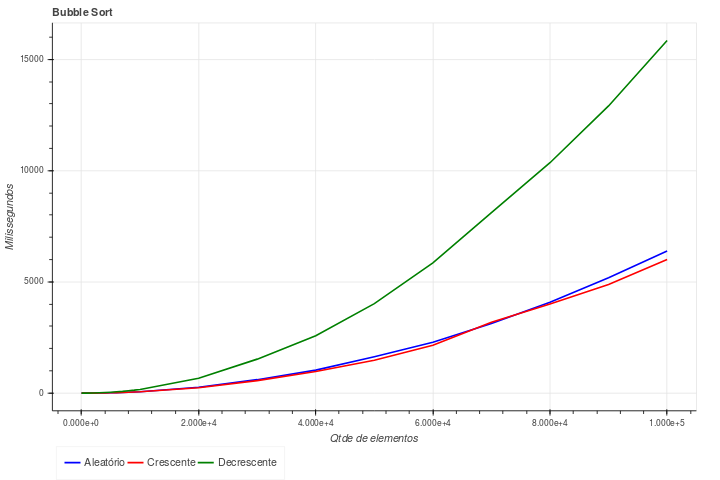
\includegraphics[scale=0.6]{img/algoritmos/bubble_sort.png}
	\caption{Bubble Sort, gráfico de resultados.}
	\label{graph-bubble}
\end{figure}

\subsection{Shell sort}
\begin{longtable}{|r|c|c|c|}
	\hline
	\csvreader[
		column count=5,
		no head,
		table head=\hline,
		late after line=\\\hline
	]{csvs/Shell_Sort.csv}{
		1=\n-elementos, 2=\aleatorio, 3=\crescente, 4=\decrescente
	}{ \n-elementos & \aleatorio & \crescente & \decrescente }
	\caption{Média de tempo do Shell Sort}
	\label{t-shell}
\end{longtable}

\begin{figure}[H]
	\centering
	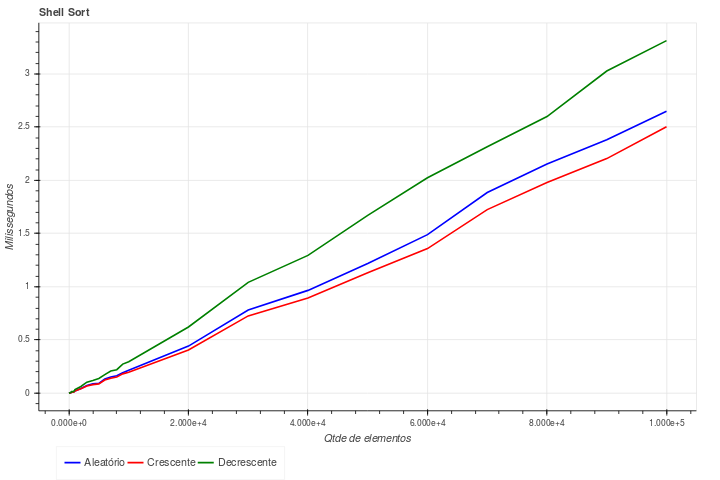
\includegraphics[scale=0.6]{img/algoritmos/shell_sort.png}
	\caption{Shell Sort, gráfico de resultados.}
	\label{graph-shell}
\end{figure}

\subsection{Quicksort}
\begin{longtable}{|r|c|c|c|}
	\hline
	\csvreader[
		column count=5,
		no head,
		table head=\hline,
		late after line=\\\hline
	]{csvs/Quicksort.csv}{
		1=\n-elementos, 2=\aleatorio, 3=\crescente, 4=\decrescente
	}{ \n-elementos & \aleatorio & \crescente & \decrescente }
	\caption{Média de tempo do Quicksort}
	\label{t-quick}
\end{longtable}

\begin{figure}[H]
	\centering
	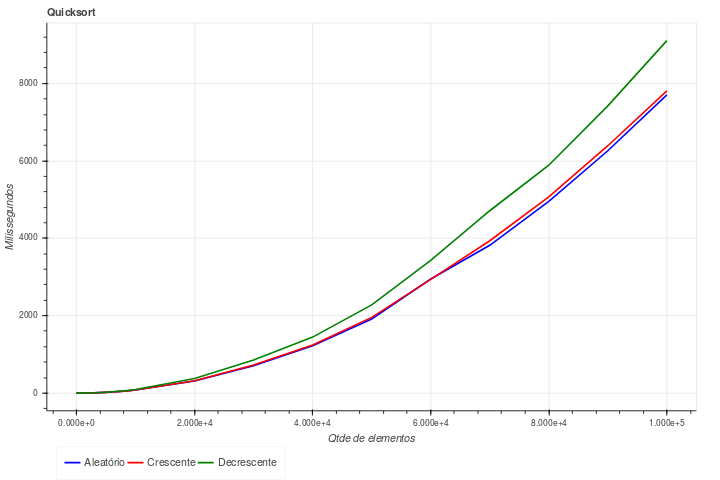
\includegraphics[scale=0.6]{img/algoritmos/quicksort.png}
	\caption{Quicksort, gráfico de resultados.}
	\label{graph-quicksort}
\end{figure}

\subsection{Merge sort}
\begin{longtable}{|r|c|c|c|}
	\hline
	\csvreader[
		column count=5,
		no head,
		table head=\hline,
		late after line=\\\hline
	]{csvs/Merge_Sort.csv}{
		1=\n-elementos, 2=\aleatorio, 3=\crescente, 4=\decrescente
	}{ \n-elementos & \aleatorio & \crescente & \decrescente }
	\caption{Média de tempo do Merge Sort}
	\label{t-merge}
\end{longtable}

\begin{figure}[H]
	\centering
	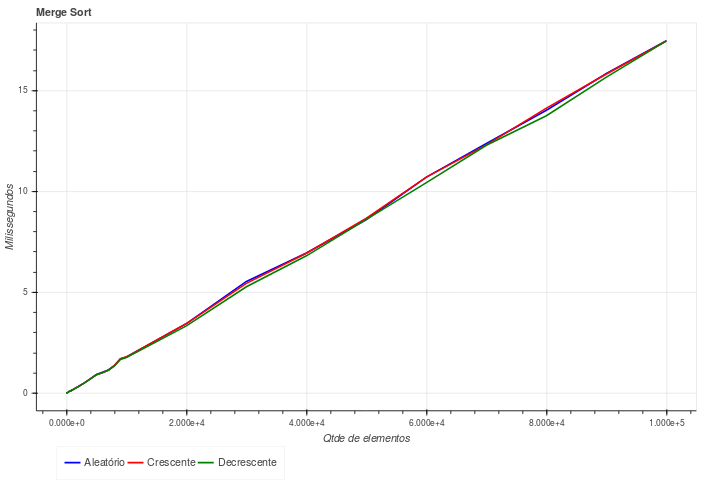
\includegraphics[scale=0.6]{img/algoritmos/merge_sort.png}
	\caption{Merge Sort, gráfico de resultados.}
	\label{graph-merge}
\end{figure}

\subsection{Radix sort (LSD)}
\begin{longtable}[c]{|r|c|c|c|}
	\hline
	\csvreader[
		column count=5,
		no head,
		table head=\hline,
		late after line=\\\hline
	]{csvs/Radix_sort_(LSD).csv}{
		1=\n-elementos, 2=\aleatorio, 3=\crescente, 4=\decrescente
	}{ \n-elementos & \aleatorio & \crescente & \decrescente }
	\caption{Média de tempo do Radix Sort (LSD)}
	\label{t-radix}
\end{longtable}

\begin{figure}[H]
	\centering
	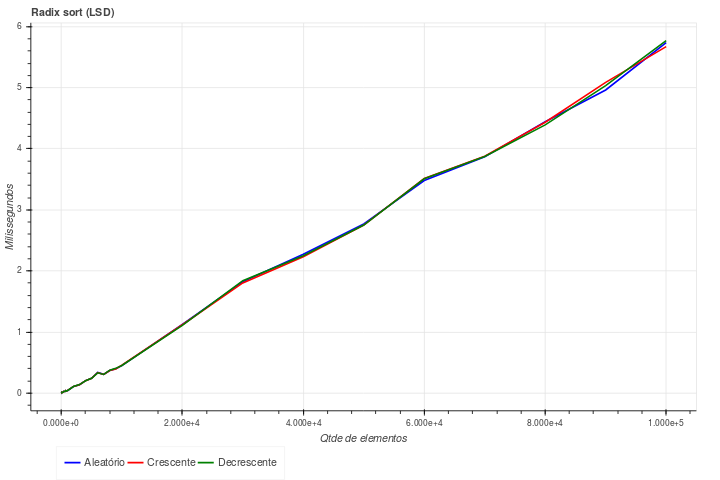
\includegraphics[scale=0.6]{img/algoritmos/radix.png}
	\caption{Radix sort (LSD), gráfico de resultados.}
	\label{graph-radix}
\end{figure}

\section{Resultados gerais}


\begin{figure}[H]
	\centering
	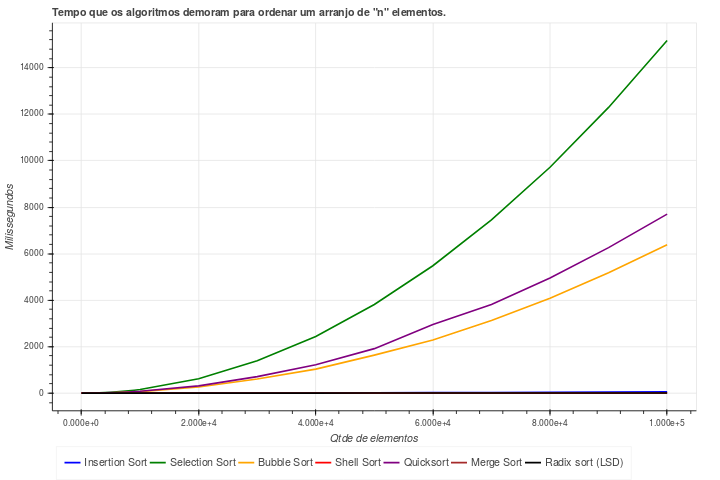
\includegraphics[scale=0.6]{img/graficos/aleatorios.png}
	\caption{Gráfico de resultados para arranjos com elementos aleatórios.}
	\label{graph-aleatorios}
\end{figure}

\begin{figure}[H]
	\centering
	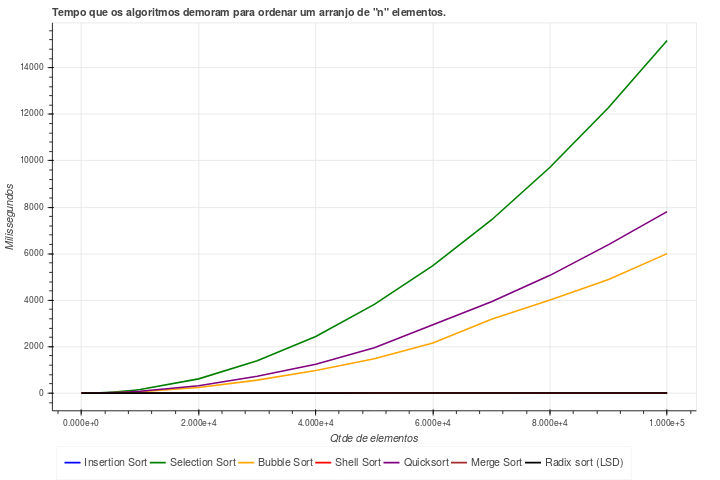
\includegraphics[scale=0.6]{img/graficos/crescentes.png}
	\caption{Gráfico de resultados para arranjos com elementos em ordem crescente.}
	\label{graph-crescentes}
\end{figure}

\begin{figure}[H]
	\centering
	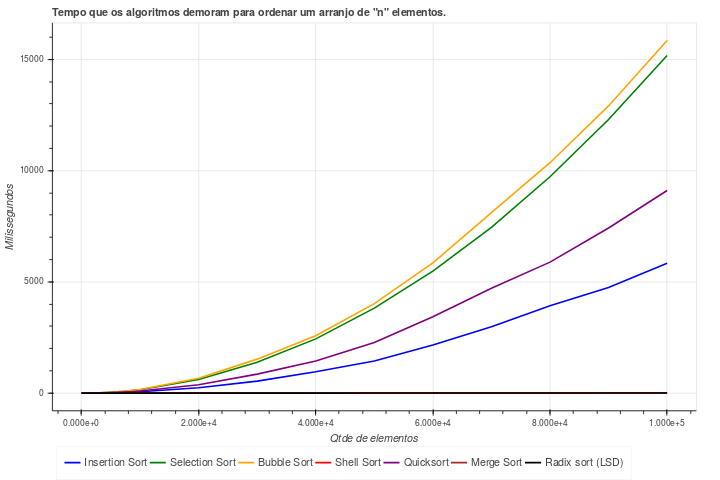
\includegraphics[scale=0.6]{img/graficos/decrescentes.png}
	\caption{Gráfico de resultados para arranjos com elementos em ordem decrescente.}
	\label{graph-decrescentes}
\end{figure}